\documentclass[10pt,xcolor={svgnames}]{beamer}
%\usefonttheme[onlymath]{serif}
%%%%% Colors
\usetheme{Dresden}%\usetheme{Madrid}
\colorlet{beamer@blendedblue}{green!55!black}
%%%%%

%%%%% Other 
\beamertemplatenavigationsymbolsempty
\addtobeamertemplate{navigation symbols}{}{%
    \usebeamerfont{footline}%
    \usebeamercolor[fg]{footline}%
    \hspace{1em}%
    \insertframenumber/\inserttotalframenumber
}
\usepackage{hyperref, url}
%\usepackage[symbol]{footmisc}

\definecolor{pine_green}{HTML}{007935}
\hypersetup{colorlinks,breaklinks,linkcolor=white,urlcolor=orange,citecolor=black}
\renewcommand\thefootnote{\textcolor{pine_green}{\arabic{footnote}}}
\setbeamercolor{alerted text}{fg=pine_green}

\renewcommand{\i}{\mathnormal{I}}

\usepackage{cancel}
\usepackage{ulem}
\usepackage{multirow}
\usepackage{mathtools}
\usepackage{makecell}
\usepackage{multicol}
\DeclarePairedDelimiter{\abs}{\lvert}{\rvert}
\renewcommand{\epsilon}{\varepsilon}
\setbeamertemplate{itemize subitem}{\textbullet}
\setbeamertemplate{itemize subsubitem}{$\circ$}

%https://tex.stackexchange.com/questions/289542/auto-resizing-parenthesis-in-math-formulas
% \usepackage{amsmath} for testing
\newcommand*\autoop{\left(}
\newcommand*\autocp{\right)}
\newcommand*\autoob{\left[}
\newcommand*\autocb{\right]}
\AtBeginDocument {%
   \mathcode`( 32768
   \mathcode`) 32768
   \mathcode`[ 32768
   \mathcode`] 32768
   \begingroup
       \lccode`\~`(
       \lowercase{%
   \endgroup
       \let~\autoop
   }\begingroup
       \lccode`\~`)
       \lowercase{%
   \endgroup
       \let~\autocp
   }\begingroup
       \lccode`\~`[
       \lowercase{%
   \endgroup
       \let~\autoob
   }\begingroup
       \lccode`\~`]
       \lowercase{%
   \endgroup
       \let~\autocb
   }}

\delimiterfactor 1001

\makeatletter
% for amsmath "compatibility" (not sophisticated)
% \usepackage{amsmath}
\AtBeginDocument {%
          \def\resetMathstrut@{%
           \setbox\z@\hbox{\the\textfont\symoperators\char40}%
           \ht\Mathstrutbox@\ht\z@ \dp\Mathstrutbox@\dp\z@}%
}%
\makeatother
%%%%%

%%%%% Greying out/invisible Slides
%\setbeamercovered{invisible}
%\setbeamercovered{%
%  again covered={\opaqueness<1->{15}}}
  
%%%%%







%%%%% Footnotes and captions
%\usepackage[utf8]{inputenc}
\usepackage{caption}
\usepackage{comment}
\setbeamerfont{footnote}{size=\tiny}
\setbeamerfont{caption}{size=\small}
%\setbeamerfont{normal text}{size=\small}
\setbeamerfont{itemize/enumerate body}{size=\small}
\setbeamerfont{itemize/enumerate subbody}{size=\footnotesize}
%%%%%


%%%%
\usepackage{booktabs}
\usepackage{multirow,bigstrut}
\usepackage{tabu}

%%%%



%Information to be included in the title page:
\title[Connor Wiegand]{Intro to Economic Analysis: Microeconomics}
\subtitle{EC 201 - Day 15 Slides}
\author[EC 201]{Connor Wiegand}
\institute[]{Department of Economics - University of Oregon}
\date{15 November 2021}


\begin{document}

\frame{\titlepage}

\section*{Note from Last Time}

\begin{frame}{Logistics}
    \begin{itemize}
        \item Homework 6 due this Saturday at 11:59pm, homework 7-8 can be flexible (up to discussion, posted date is final)
        \item I will post final news assignments soon, the final news assignment is due next Wednesday (Nov 24) at 11:59pm
        \item Midterm discussion at end of class
    \end{itemize}
\end{frame}


\begin{frame}{Positive Consumption Externality}
    \begin{itemize}[<+->]
        \item Recall the Vegan Food Example
        \item Here is the CS, PS, and EB (i.e., TS) before the subsidy:
        \begin{figure}
            \centering
            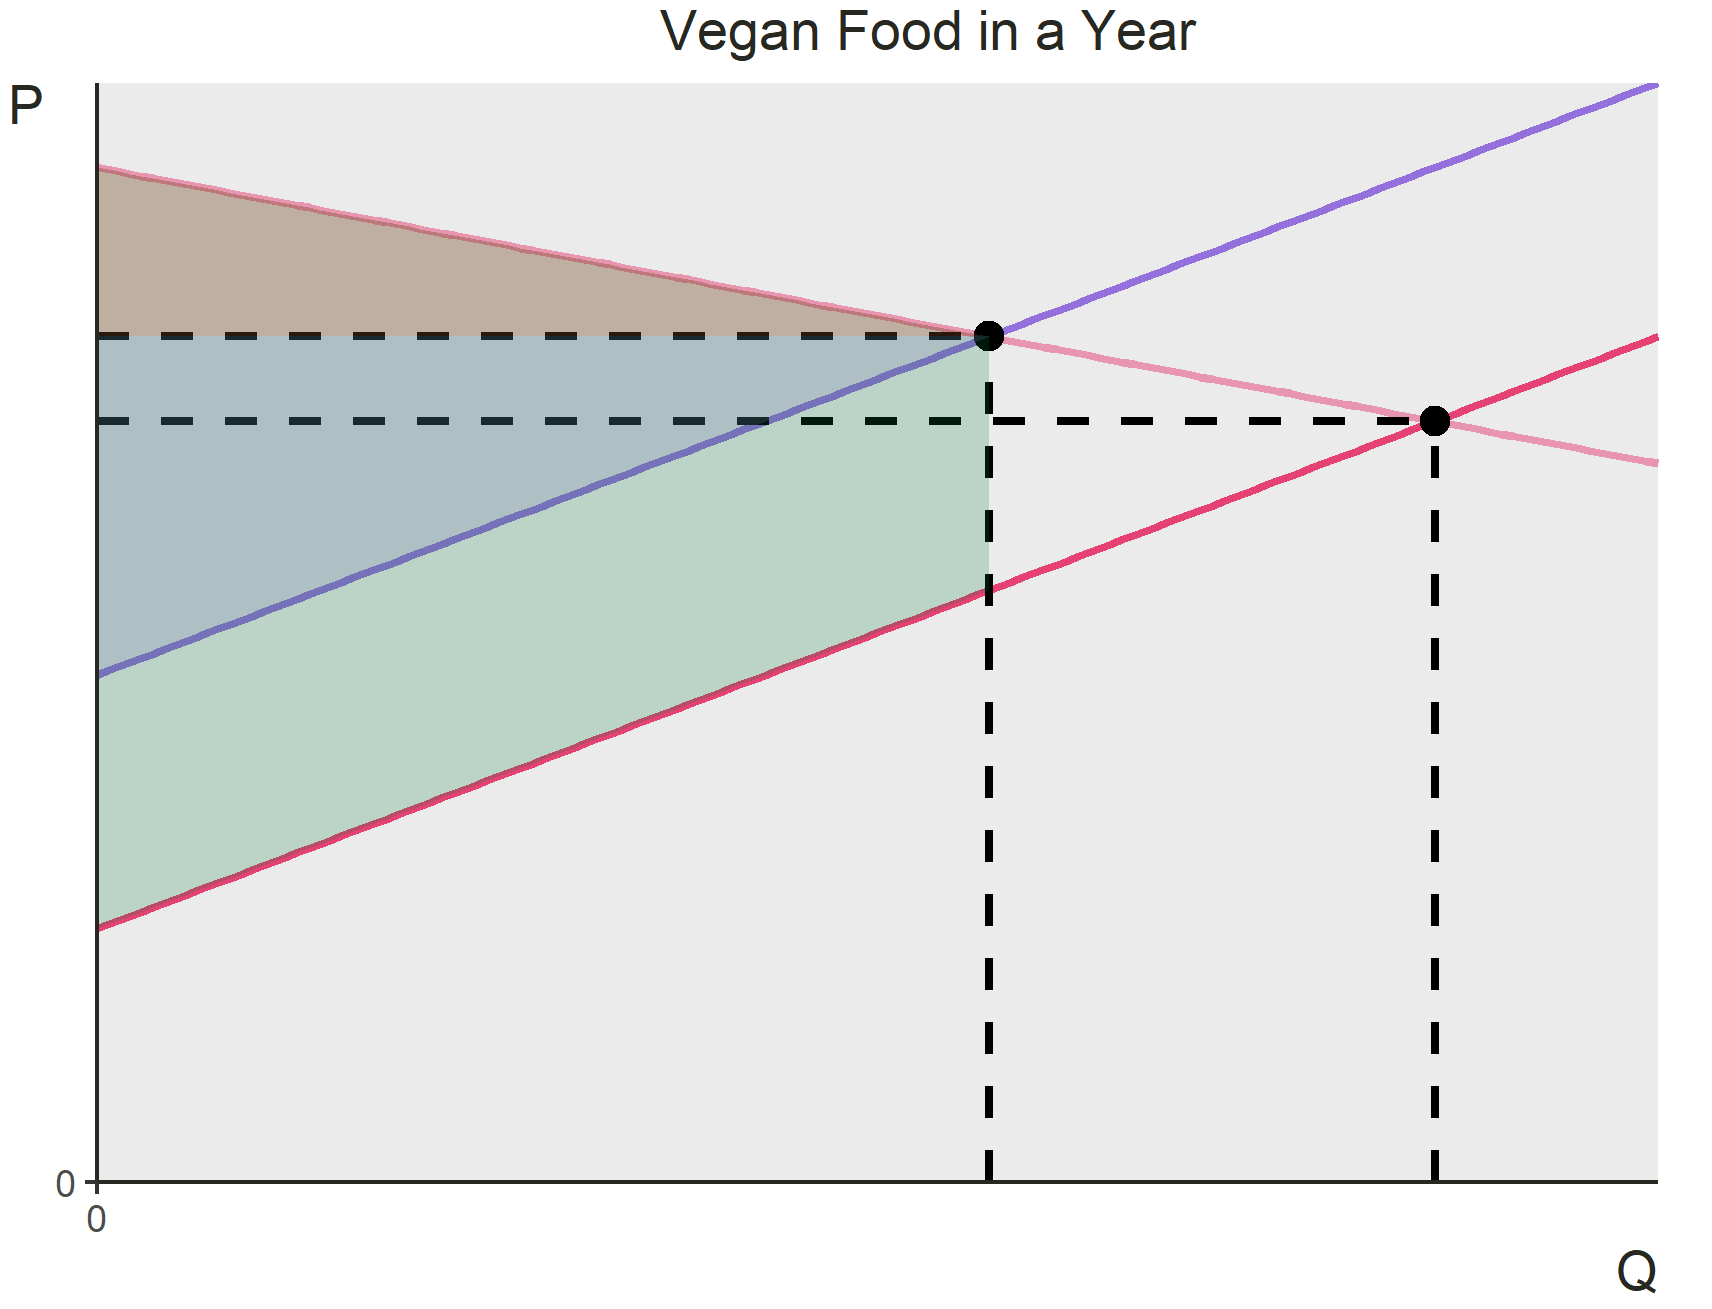
\includegraphics[width=7.5cm]{cpext ts.png}
        \end{figure}
    \end{itemize}
\end{frame}

\begin{frame}{Positive Consumption Externality}
    \begin{itemize}[<+->]
        \item With a $\$4000$ subsidy, demand becomes MSB:
        \begin{figure}
            \centering
            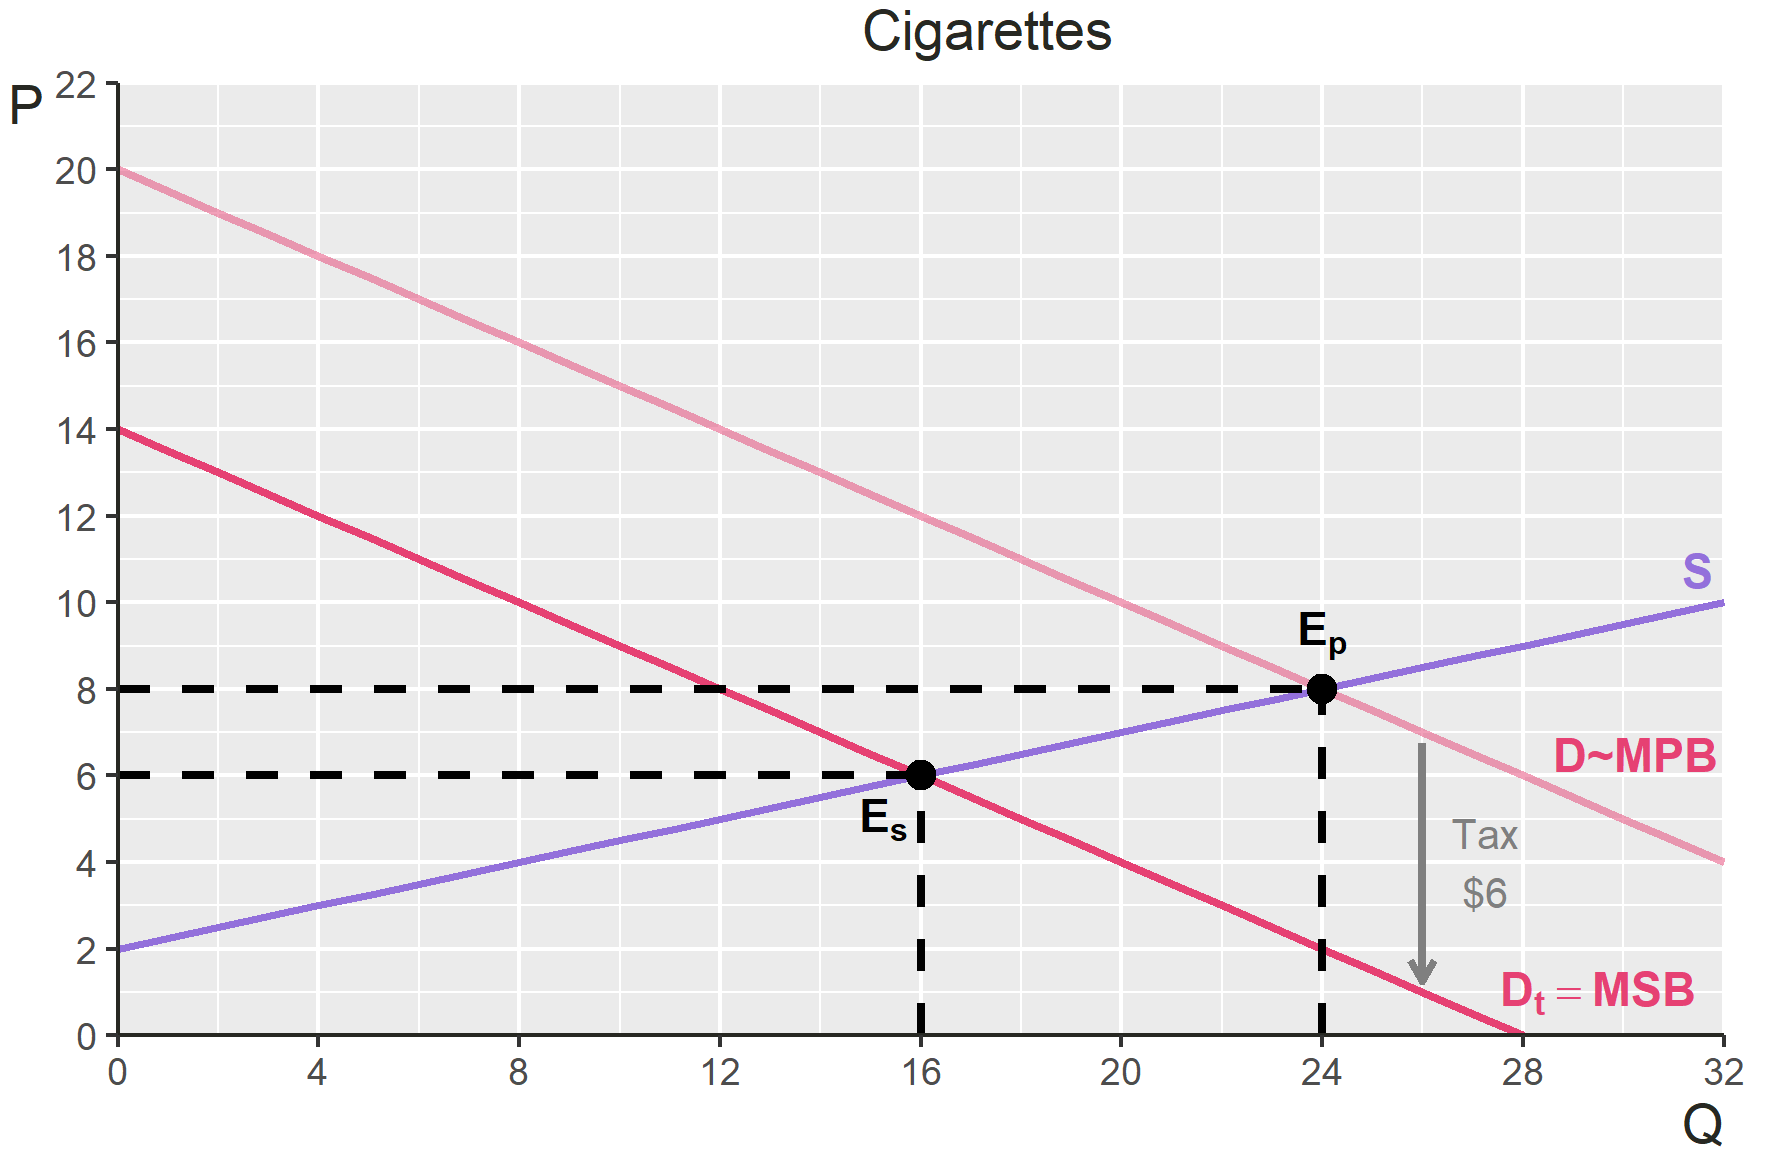
\includegraphics[width=7cm]{cnext tax base.png}
        \end{figure}
    \end{itemize}
\end{frame}

\begin{frame}{Positive Consumption Externality}
    \begin{itemize}[<+->]
        \item The EB is now given by
        \begin{figure}
            \centering
            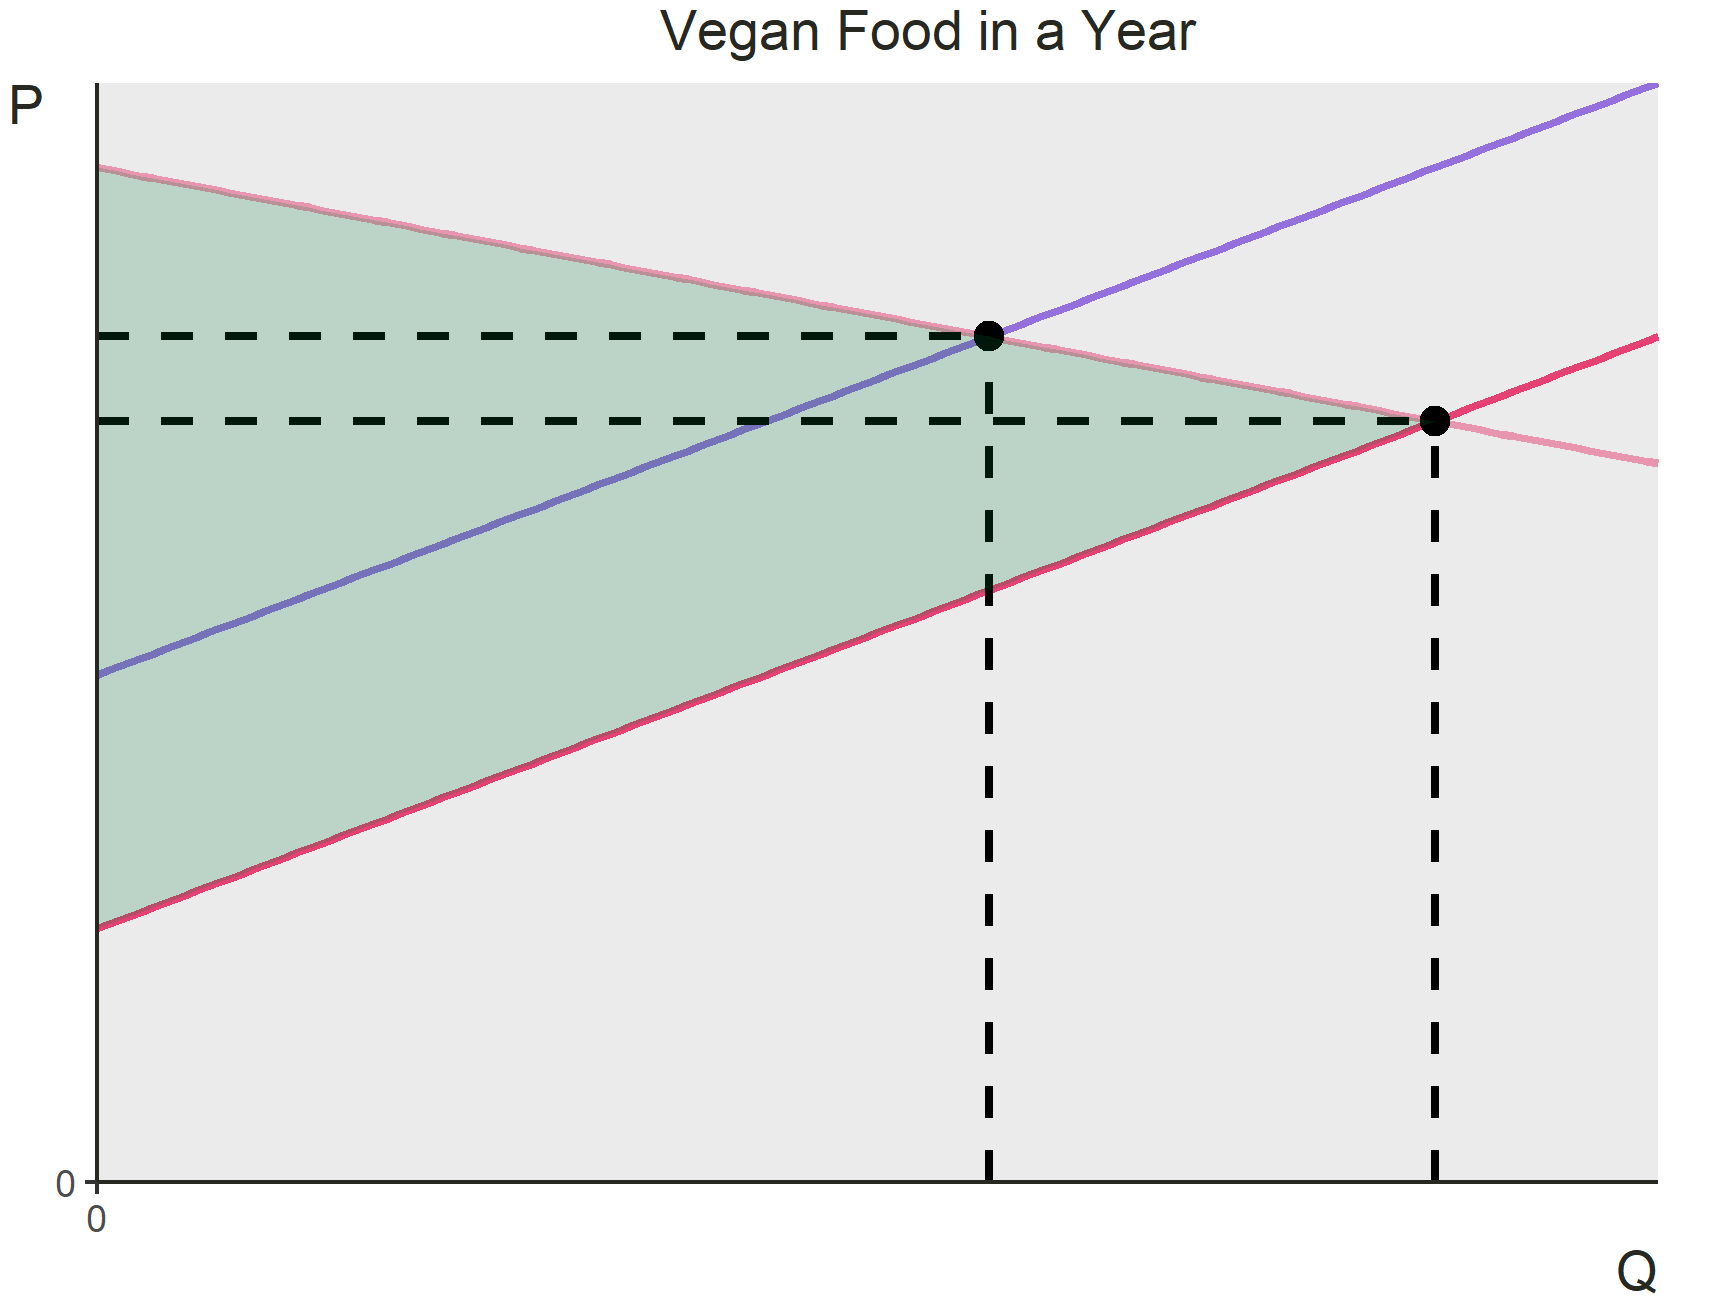
\includegraphics[width=7cm]{cpext tax eb.png}
        \end{figure}
        $$EB=(12000)(14000-10000)=48M$$
    \end{itemize}
\end{frame}

\begin{frame}{Positive Consumption Externality}
    \begin{itemize}[<+->]
        \item And now, we have some GE
        \begin{figure}
            \centering
            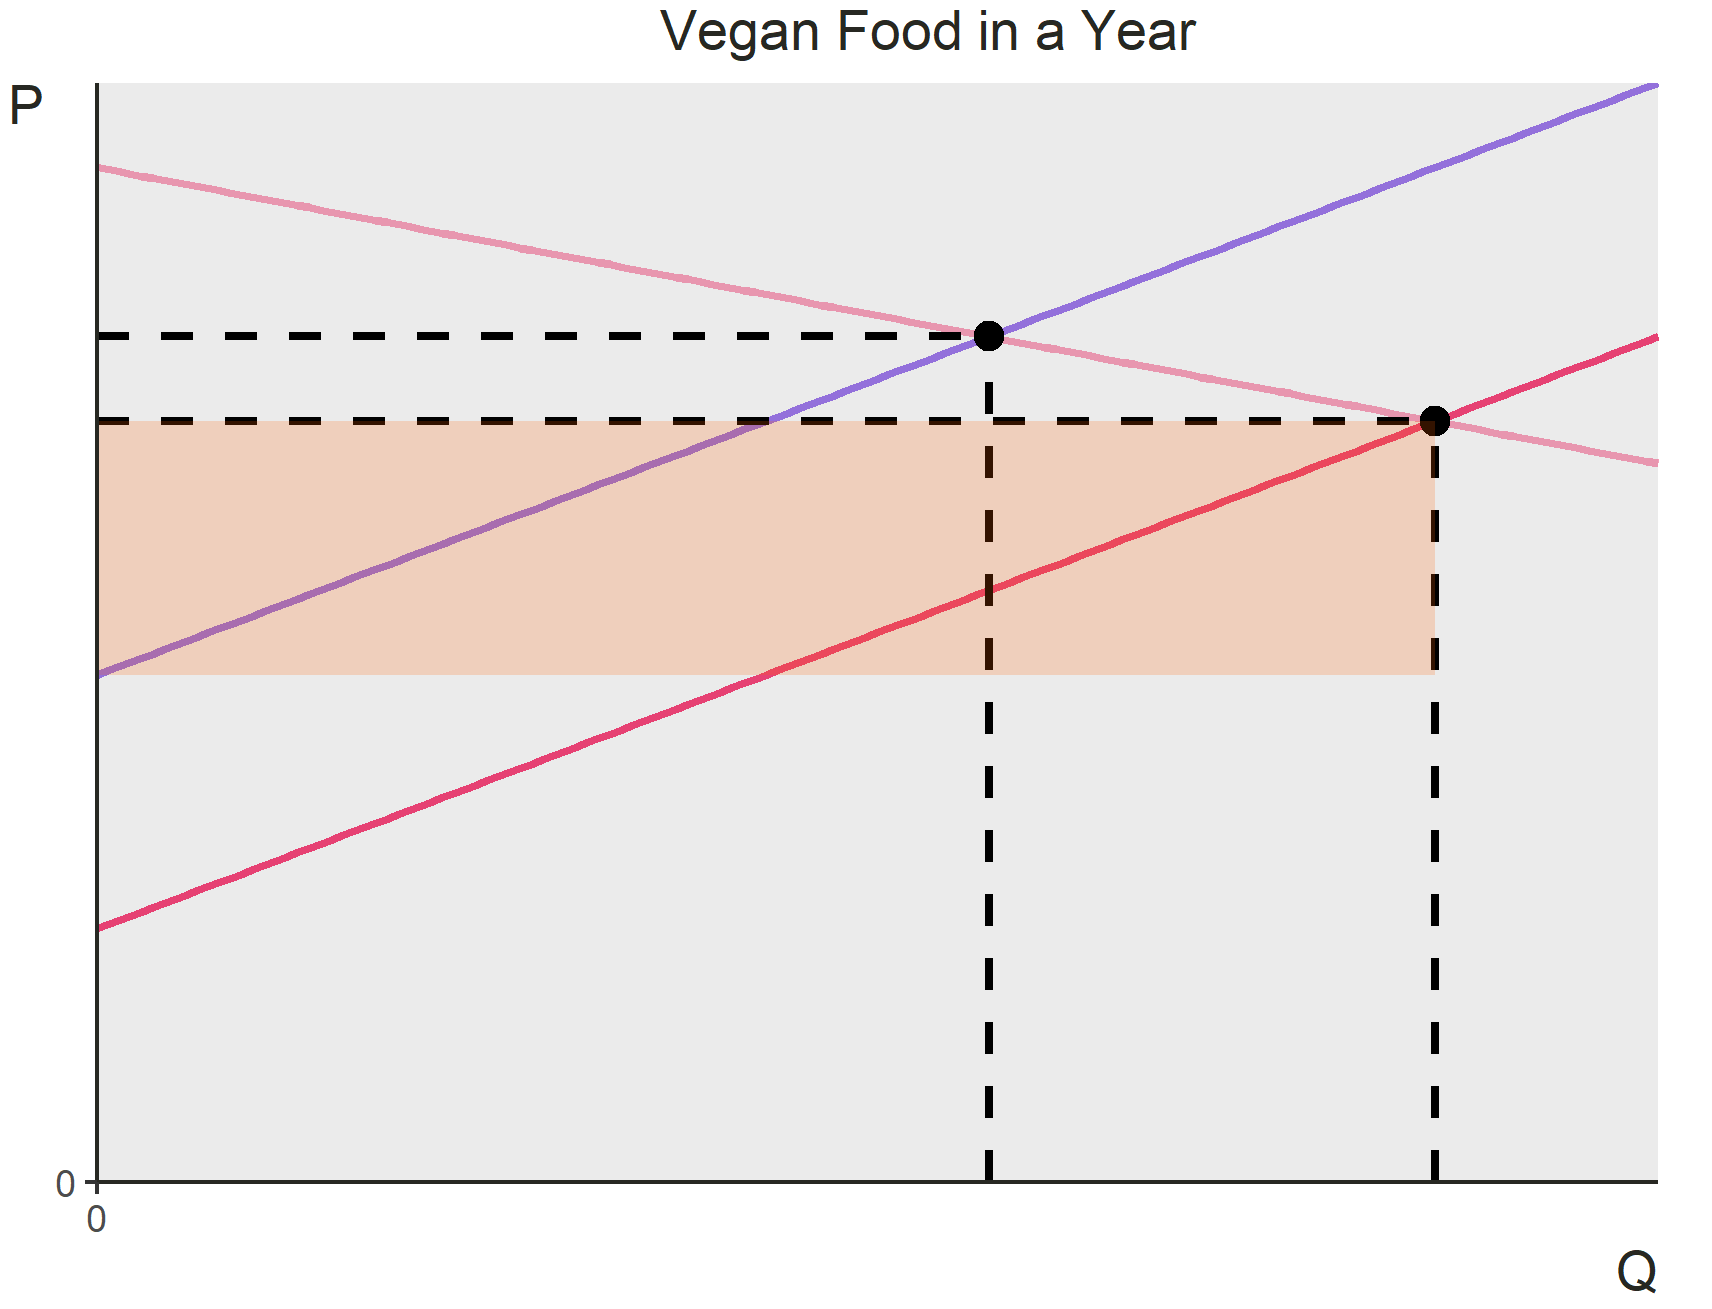
\includegraphics[width=7cm]{cpext tax ge.png}
        \end{figure}
        $$GE=(12000)(8000-4000)=48M$$
    \end{itemize}
\end{frame}

\begin{frame}{Positive Consumption Externality}
    \begin{itemize}[<+->]
        \item After EB and GE cancel out, only CS and PS make up TS\footnote{Of course, that's \underline{not} to say that EB and GE don't count towards TS, they just cancel out}
        \begin{figure}
            \centering
            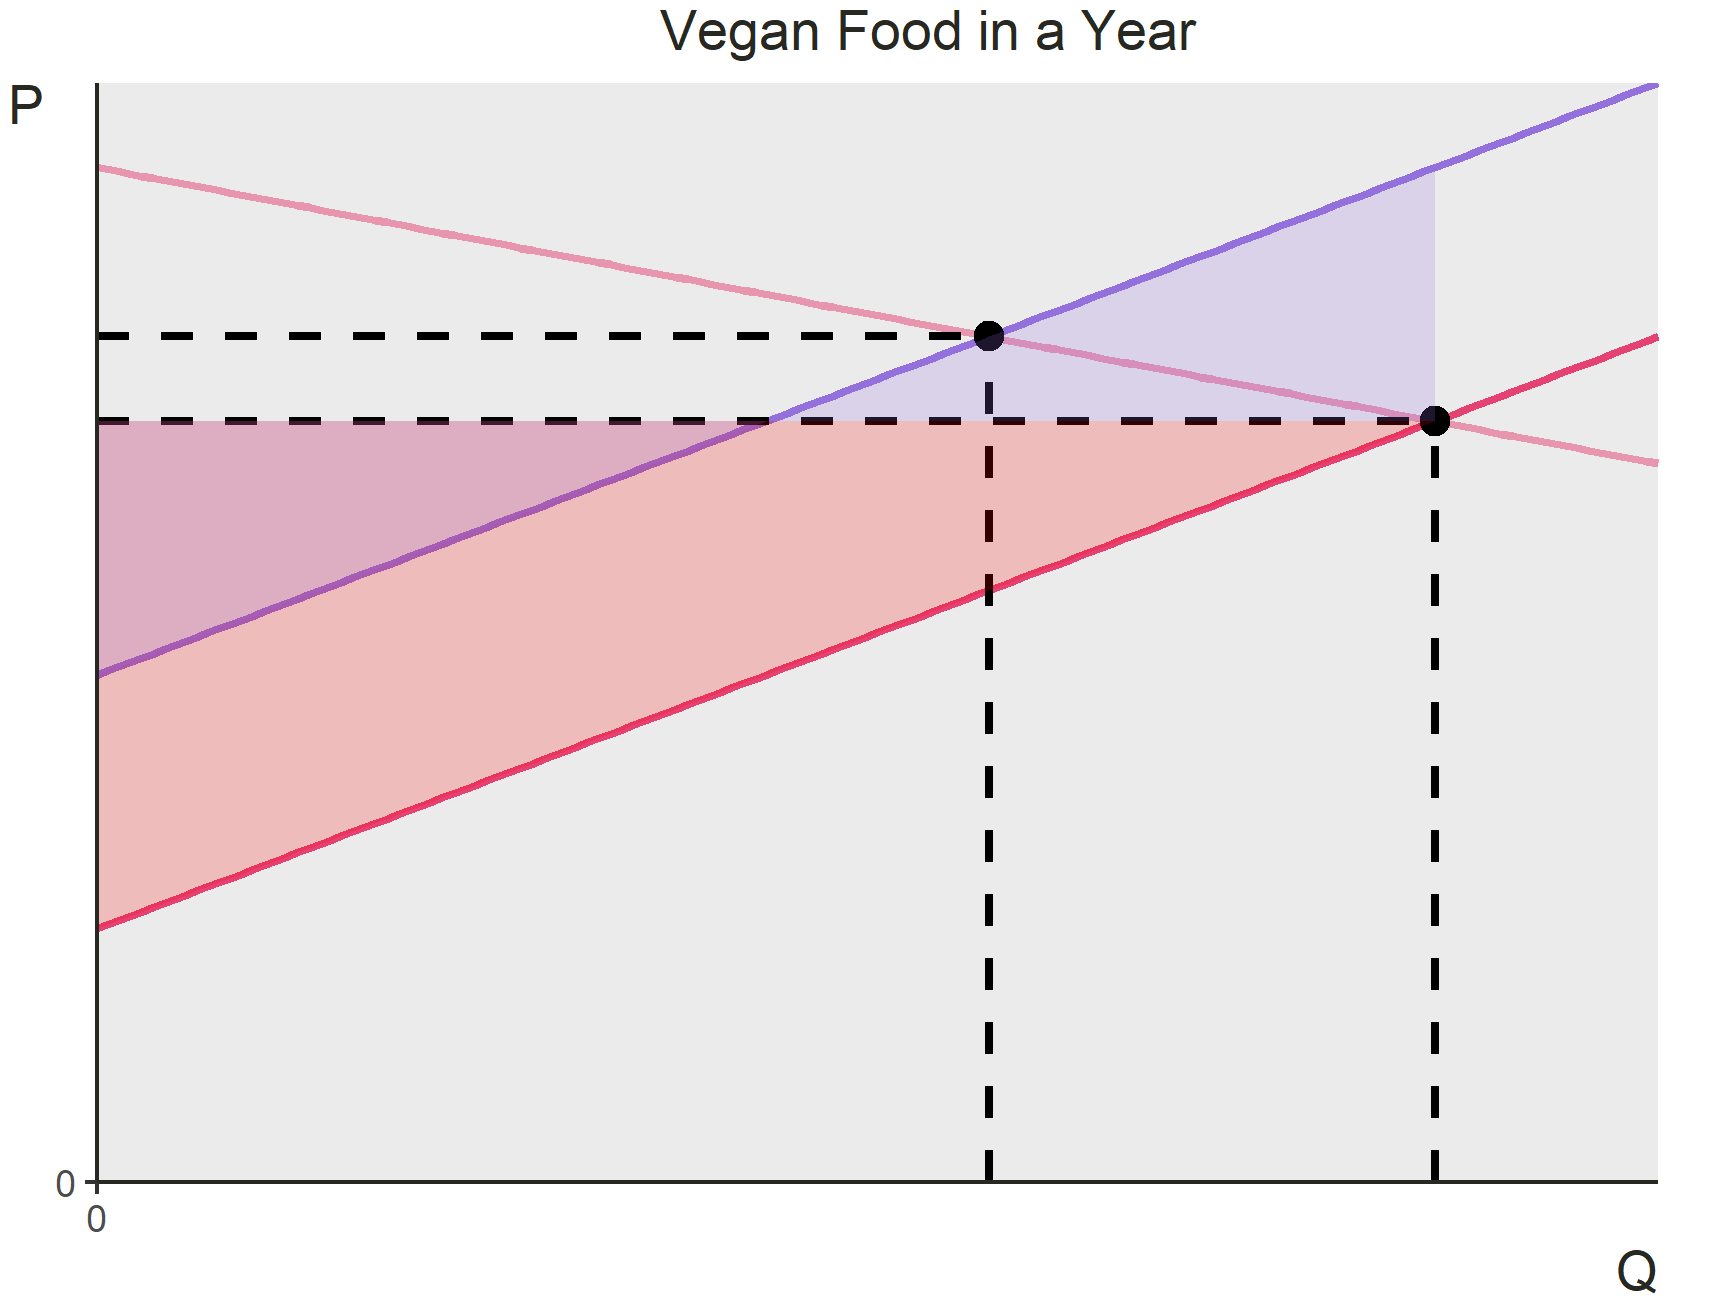
\includegraphics[width=7cm]{cpext tax csps.png}
        \end{figure}
    \end{itemize}
\end{frame}

\begin{frame}{Positive Consumption Externality}
    \begin{itemize}[<+->]
        \item Thus, the only numerical difference -- which is DWL -- is the following triangle
        \begin{figure}
            \centering
            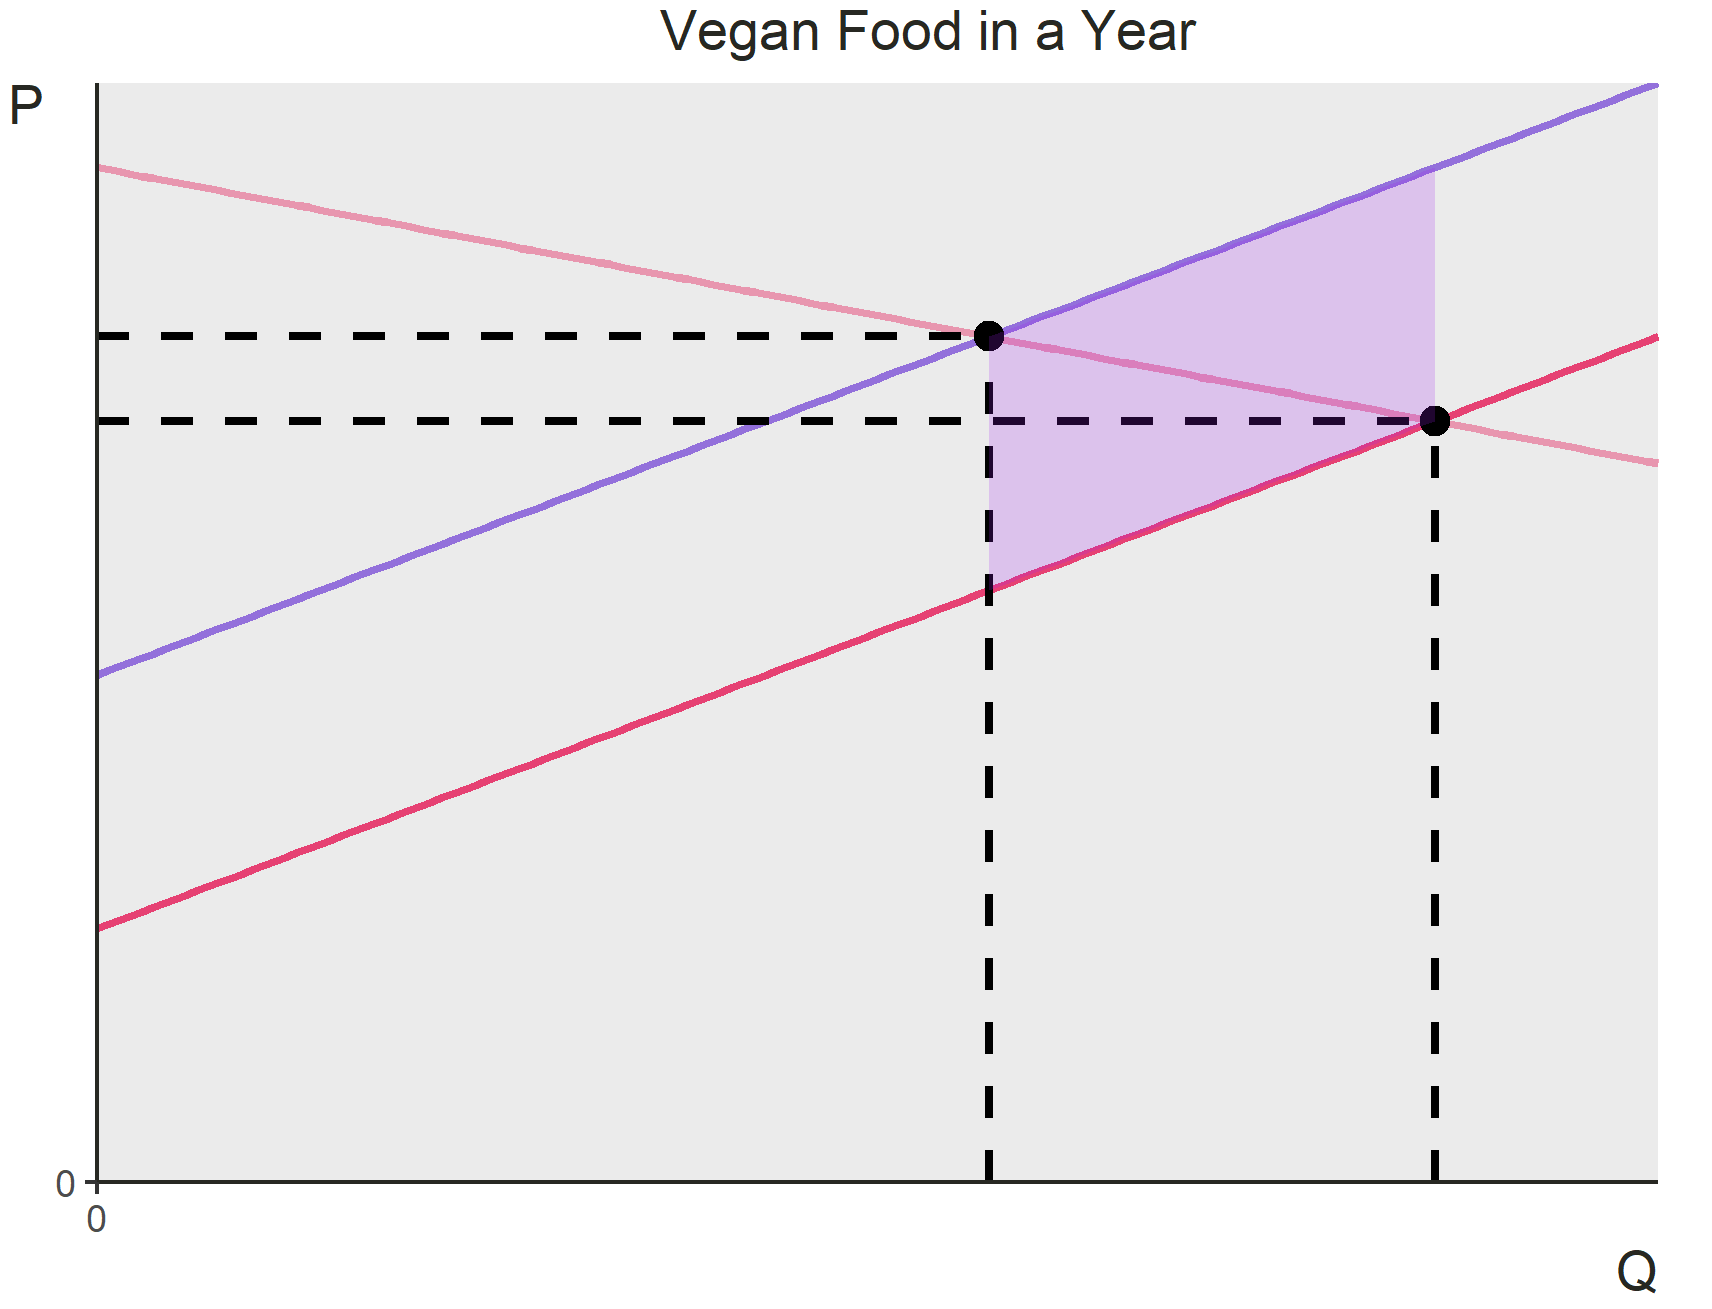
\includegraphics[width=7cm]{cpext dwl.png}
        \end{figure}
        $$DWL=\frac{1}{2}(12000-7200)(10400-6400)=9.6M$$
    \end{itemize}
\end{frame}

\section*{Theory of the Firm}

\begin{frame}{Where Supply Comes From}
    \begin{itemize}[<+->]
        \item We a pretty intuitive sense of where demand comes from -- \textit{valuation}
        \item When I motivated the supply curve, I just said that WTA loosely came from \textit{costs}
        \begin{itemize}
            \item When $Q$ increases, firms have to pay for more space, more labor, more machines, etc.
        \end{itemize}
        \item Now, we want to explore that concept more in depth
    \end{itemize}
\end{frame}

\begin{frame}{}
        \begin{figure}
            \centering
            
\includegraphics[width=9.5cm]{Business class meme.jpg}
        \end{figure}
\end{frame}

\begin{frame}{Economic Profit}
    \begin{itemize}[<+->]
        \item $profit =  revenue - costs$
        \item More specifically, 
        $$\pi=TR-TC$$
        where 
        \begin{itemize}
            \item $\pi$=profits
            \item TR=total revenue
            \item TC=total costs
        \end{itemize}
        \item Total revenue is exactly how we have defined it before: how many goods you sell times the price you sell them at
        \item For total cost, however, We need to be careful; there are two kinds of costs we could be talking about: \textit{accounting} costs vs \textit{economic costs}
    \end{itemize}
\end{frame}

\begin{frame}{Accounting Costs vs Economic Costs}
    \begin{itemize}[<+->]
        \item I will start by noting that this will be an important \textit{conceptual} point to understand, but it will not be a huge worry once we start going into problems\footnote{Later on, I will make this more clear}
        \item \underline{\textbf{Explicit Costs}} are tangible costs that the firm faces must pay for with real money
        \item \underline{\textbf{Implicit Costs}} are costs that the firm faces which do not require the real payment of funds
        \begin{itemize}
            \item Most often, these are \textit{opportunity costs}
        \end{itemize}
        \item \underline{\textbf{Accounting Costs}} refers to the sole consideration of explicit costs, giving rise to \underline{\textbf{Accounting Profit}}, which is simply $total\ revenue - explicit\ costs$
        \item \underline{\textbf{Economic Costs}} refers to factoring in both explicit costs and implicit costs, which gives rise to \underline{\textbf{Economic Profit}}: $total\ revenue - explicit\ costs - implicit\ costs$
    \end{itemize}
\end{frame}

\begin{frame}{Types of Profit Example}
    \begin{itemize}[<+->]
        \item Jake G's scarves sells 100 scarves a month at a price of \$20
        \item Jake G pays \$5 in materials and \$10 in labor for each scarf made
        \item Instead of selling scarves, Jake G could also take acting classes, which would cost \$250/month, but would pull in \$1000/month in revenue.
        \item Q1: What is Jake's accounting profit in one year, assuming he makes scarves?
        \begin{itemize}
            \item Per month, Jake has a TR of $100(20)=\$2000$. He faces a cost of $100(5+10)=\$1500$
            \item Per month he makes $\$500$. Per year he makes $(500)(12)=\$6000$
        \end{itemize}
        \item Q2: What is Jake's \textit{economic} profit in one year, assuming he makes scarves?
        \begin{itemize}
            \item If Jake acts, it would make him a profit of $1000-250=\$750$/month
            \item Thus, Jake's opportunity cost of making scarves is $\$750$. 
            \item Jake therefore makes $500-750=-\$250$/month, i.e. $(-250)(12)=-\$3000$/year, in economic profit
        \end{itemize}
    \end{itemize}
\end{frame}

\begin{frame}{Context for Economic Profit}
    \begin{itemize}[<+->]
        \item The takeaway from the previous example is that the accounting can be happy knowing profits are positive, when the decision could still be bad in the eyes of an economist, since the firm could make more money doing something else
        \item Note that economic profit could very well be positive, this just means that the ``next best thing" doesn't make as much as the current job/project does
        \item This is an important thing to keep in mind, and you will get problems on it here and there
        \item However, our discussion of costs from here will mostly include explicit costs and ignore implicit ones 
        \begin{itemize}
            \item However, in the background, we are assuming we are talking about economic profit in this class, rather than accounting profit, and that implicit costs are already being factored in
        \end{itemize}
    \end{itemize}
\end{frame}

\begin{frame}{Production Table}
    \begin{itemize}[<+->]
        \item The following table shows an example \underline{\textbf{production function}}: the relationship between the quantity of inputs used to make a good and the quantity of output of that good
        \begin{table}[]
            \centering
            \begin{tabular}{c|c|c|c}
                \thead{\textbf{\# Workers}\\ (Labor)} & \thead{\textbf{\# of $x$}\\ (Output)} & \thead{\textbf{Startup Costs}\\ (Fixed Cost)} & \thead{\textbf{Wage}\\ (Cost of Labor)} \\ 
                \hline
                0 & 0.0 & \$50 & \$10 \\
                1 & 4.0 & \$50 & \$10\\
                2 & 5.6 & \$50 & \$10\\
                3 & 6.9 & \$50 & \$10 \\
                4 & 8.0 & \$50 & \$10\\
                5 & 8.9 & \$50 & \$10\\
                6 & 9.7 & \$50 & \$10\\
                7 & 10.5 & \$50 & \$10\\
                8 & 11.3 & \$50 & \$10 \\
                9 & 12.0 & \$50 & \$10
                \end{tabular}
        \end{table}
    \end{itemize}
\end{frame}

\begin{frame}{Production Function}
    \begin{itemize}[<+->]
        \item The aforementioned table, when graphing output to \# workers, induces the following graph of the firm's production function:
        \begin{figure}
            \centering
            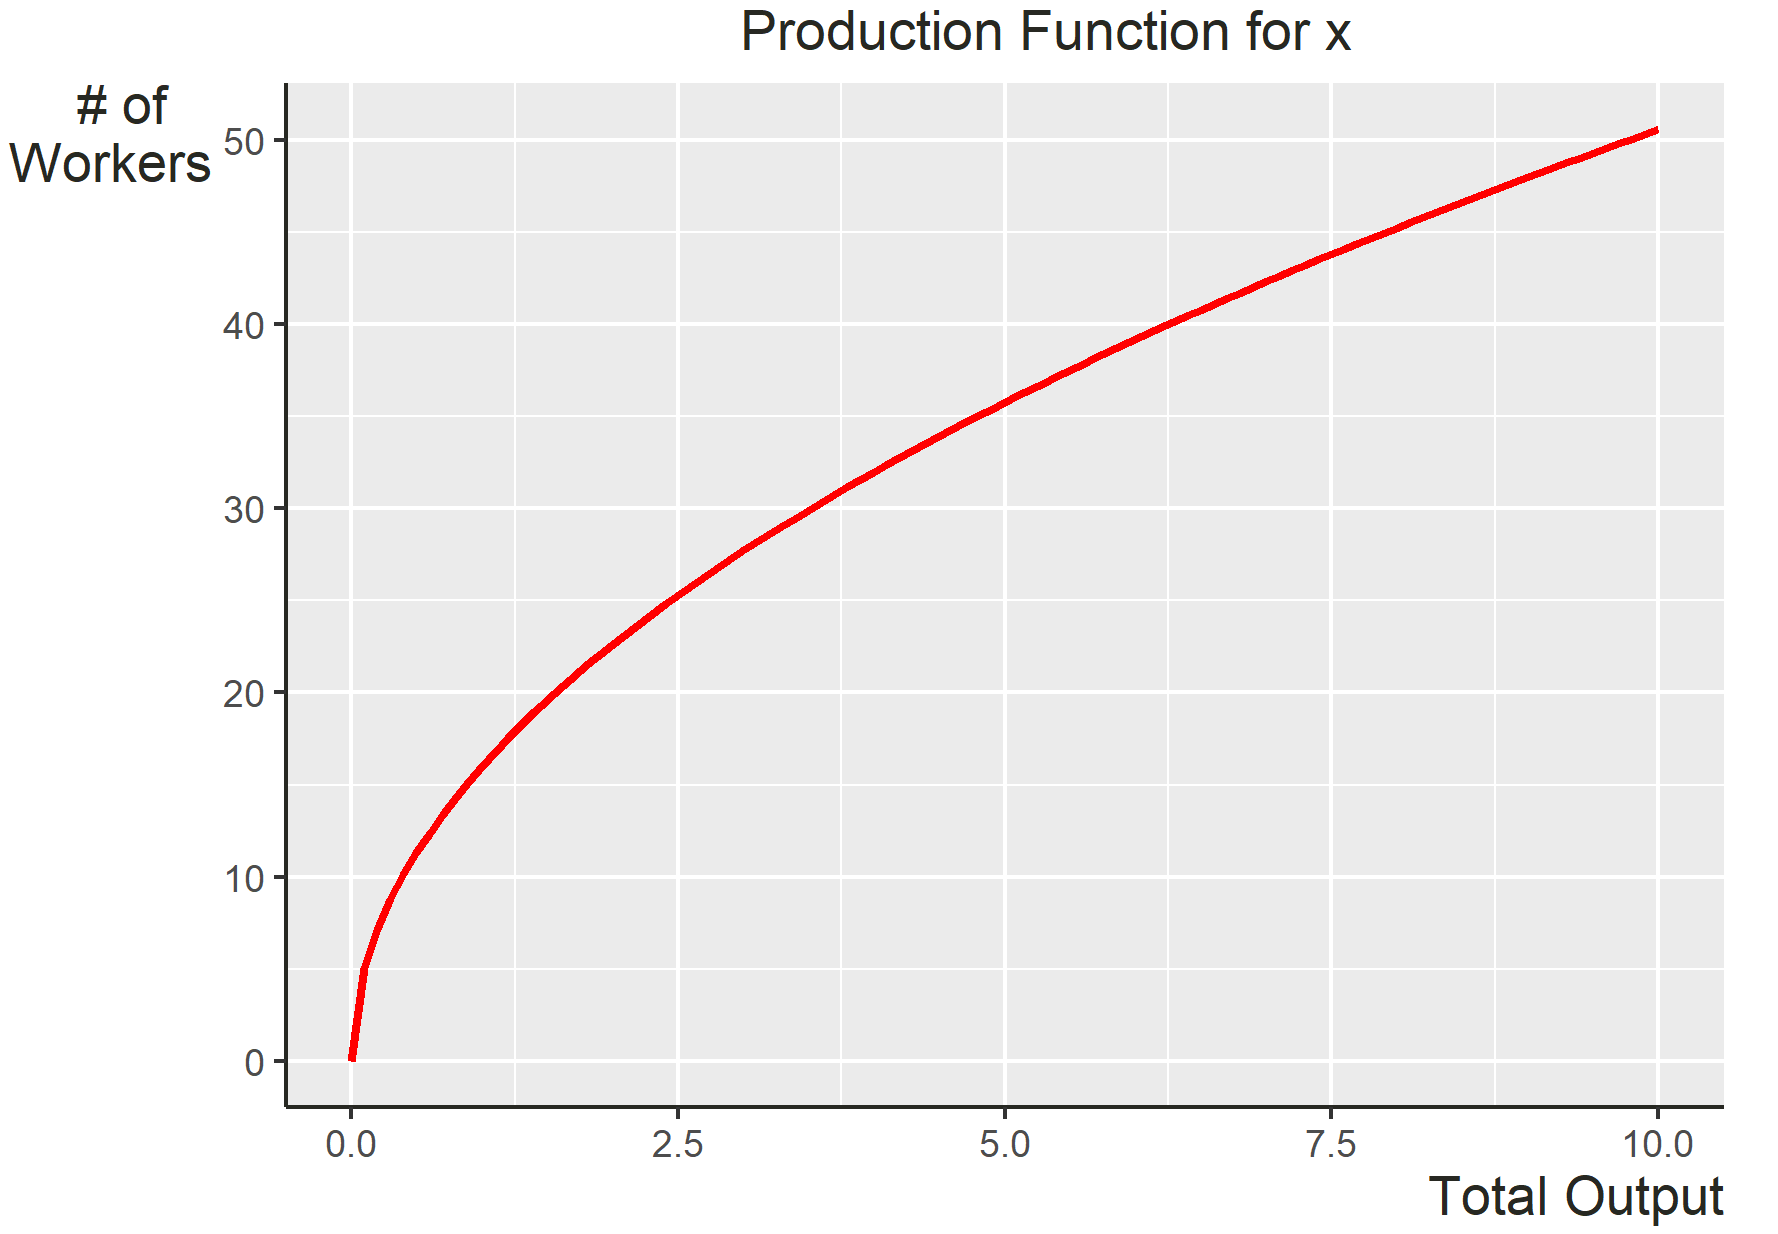
\includegraphics[width=7cm]{PF1.png}
        \end{figure}
        \item Note how the curve flattens out (i.e., the slope diminishes) as $Q$ increases
    \end{itemize}
\end{frame}

\begin{frame}{Marginal Products}
    \begin{itemize}[<+->]
        \item The first concept we must discuss is the idea of \textit{marginal product}
        \begin{itemize}
            \item This will play a minor role in our overall discussion, but is a key concept to understand
        \end{itemize}
        \item Simply put, the \underline{\textbf{marginal product}} of an input is the increase in output that arises from an additional unit of that input
        \item In economics, the two key marginal products are the \underline{marginal product of labor} ($MP_{L}$) and the \underline{marginal product of capital} ($MP_{K}$)
        \begin{itemize}
            \item This is because we often times want to ask what the trade off is behind hiring another worker (labor) and buying/renting a new machine (capital)
        \end{itemize}
        \item If we have one input, then the slope of the production function will equal the marginal product of that input
        \begin{itemize}
            \item In fact, if we graph output to any input, then the slope of that curve will be the marginal product of that input
        \end{itemize}
    \end{itemize}
\end{frame}

\begin{frame}{Production Table}
    \begin{itemize}[<+->]
        \item The following table now shows the marginal product of labor
        \begin{table}[H]
            \centering
            \begin{tabular}{c|c|c|c|c}
                \thead{\textbf{\# Workers}\\ (Labor)} & \thead{\textbf{\# of $x$}\\ (Output)} & \thead{\textbf{Startup Costs}\\ (Fixed Cost)} & \thead{\textbf{Wage}\\ (Cost of Labor)} & \thead{$MP_{L}$\\ \ } \\ 
                \hline
                0 & 0.0 & \$50 & \$18 & ---\\
                1 & 4.0 & \$50 & \$18 & 4.0\\
                2 & 5.6 & \$50 & \$18 & 1.6\\
                3 & 6.9 & \$50 & \$18 & 1.3\\
                4 & 8.0 & \$50 & \$18 & 1.1\\
                5 & 8.9 & \$50 & \$18 & 0.9\\
                6 & 9.7 & \$50 & \$18 & 0.8\\
                7 & 10.5 & \$50 & \$18 & 0.8\\
                8 & 11.3 & \$50 & \$18 & 0.8\\
                9 & 12.0 & \$50 & \$18 & 0.7
                \end{tabular}
        \end{table}
                \item As each extra worker is hired, the contribute fewer $x$. What is this called?
        \begin{itemize}
            \item \textit{Diminishing marginal returns}, a concept we have seen before
            \item While we may see increasing or constant MPs, economists believe that eventually a firm will experience diminishing marginal products
        \end{itemize}
    \end{itemize}
\end{frame}


\begin{frame}{Marginal Thinking}
    \begin{itemize}[<+->]
        \item Suppose the price of $x$ is $\$20$, and we can sell all of our output. How many workers should we hire?
        \item Suppose we've hired three workers. Should we hire a fourth?
        \begin{itemize}
            \item The fourth worker will cost \$18, but will earn us $1.1(\$20)=\$22$: they are worth the hire! 
        \end{itemize}
        \item Suppose we've hired four workers. Should we hire a fifth?
        \begin{itemize}
            \item The fifth worker will cost \$18, and will earn us $0.9(\$20)=\$18$: they are barely worth the hire
            \item We will say they are worth it, because if we consider a continuum of workers (maybe via hiring part time), then the 4.9th worker will be worth it, as will be the 4.95th, etc. 
        \end{itemize}
        \item Should we hire any more?
        \begin{itemize}
            \item The fourth worker will cost \$18, but will only earn us $1.8(\$20)=\$16$: they are not worth it
        \end{itemize}
        \item Thus, we should hire 5 workers
    \end{itemize}
\end{frame}

\begin{frame}{Marginal Thinking(cont.)}
    \begin{itemize}[<+->]
        \item In this example, we should hire up until marginal product times price equals the wage (which is also the marginal cost) of labor
        \item This idea of having marginal things equal each other will be a key idea for us in the coming chapters
        \item The idea will always be the same: if it's profitable to keep going, keep going; if we are losing profit, go back; if we break even, we are right on the sweet spot
    \end{itemize}
\end{frame}

\begin{frame}{Total Costs}
    \begin{itemize}[<+->]
        \item The production table also generates for us a \textit{total cost} column, shown below
        \begin{table}[H]
            \centering
            \begin{tabular}{c|c|c|c|c}
                \thead{\textbf{\# Workers}\\ (Labor)} & \thead{\textbf{\# of $x$}\\ (Output)} & \thead{\textbf{Startup Costs}\\ (Fixed Cost)} & \thead{\textbf{Wage}\\ (Cost of Labor)} & \thead{\textbf{Total Cost}\\ \ } \\ 
                \hline
                0 & 0.0 & \$50 & \$18 & \$50\\
                1 & 4.0 & \$50 & \$18 & \$68\\
                2 & 5.6 & \$50 & \$18 & \$86\\
                3 & 6.9 & \$50 & \$18 & \$104\\
                4 & 8.0 & \$50 & \$18 & \$122\\
                5 & 8.9 & \$50 & \$18 & \$140\\
                6 & 9.7 & \$50 & \$18 & \$158\\
                7 & 10.5 & \$50 & \$18 & \$176\\
                8 & 11.3 & \$50 & \$18 & \$194\\
                9 & 12.0 & \$50 & \$18 & \$212
                \end{tabular}
        \end{table}
    \end{itemize}
\end{frame}

\section*{Costs}

\begin{frame}{Total Cost Curve}
    \begin{itemize}[<+->]
        \item Plotting Total Cost against output yields our total cost curve:
        \begin{figure}
            \centering
            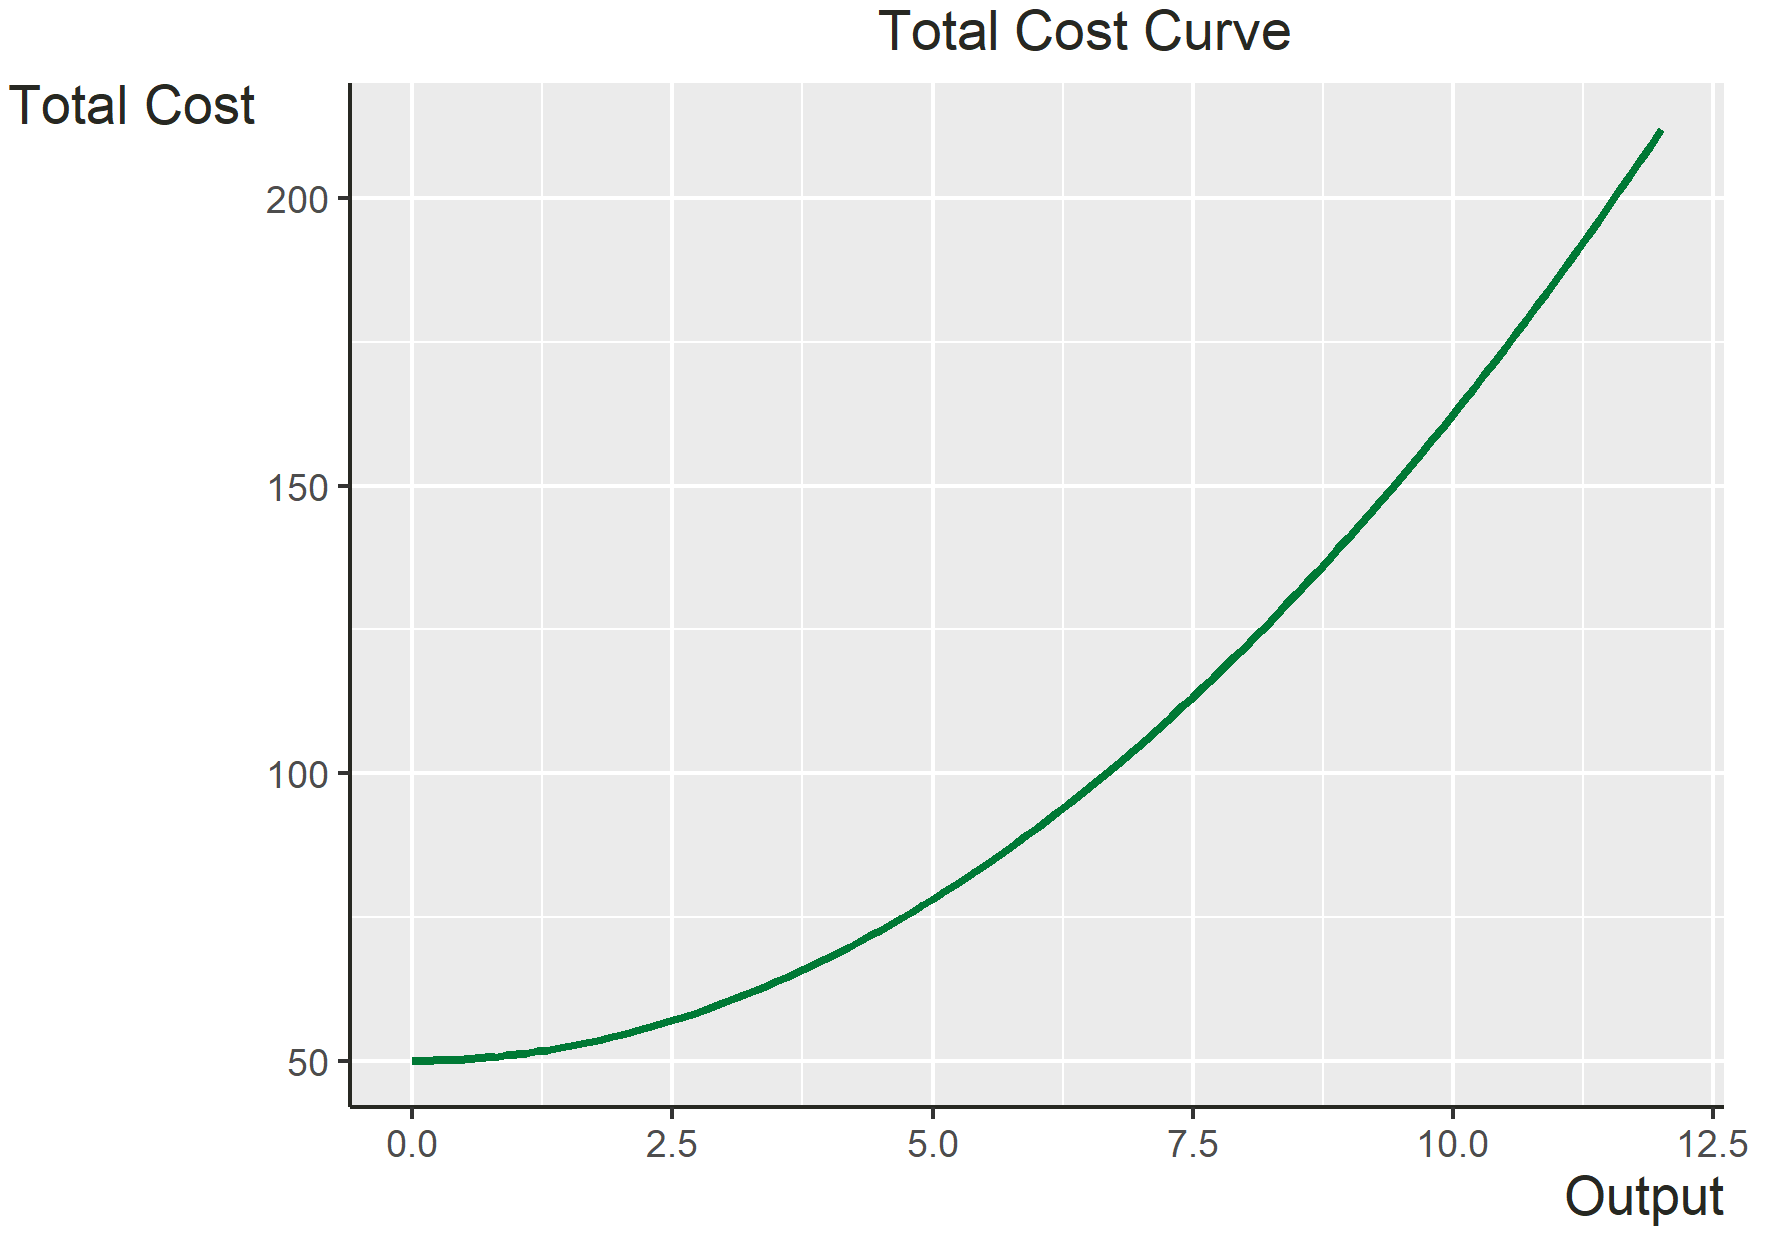
\includegraphics[width=7cm]{TC1.png}
        \end{figure}
        \item Note: the total cost curve slopes upward (and eventually becomes exponential) because of diminishing marginal returns in the production function
    \end{itemize}
\end{frame}

\begin{frame}{From Production to Costs}
    \begin{itemize}[<+->]
        \item The production function is important determining how a business produces output
        \item Once we know the production function and the price, however, we really just need to know costs, and a lot of things go into cost
        \item In fact, the total cost curve and the production function curve carry a lot of the same information
        \begin{itemize}
            \item The total cost curve gets steeper as the amount produced rises, whereas the production function gets flatter as production rises. These changes in slope occur for the same reason:
            \begin{itemize}
                \item  High production of $x$ means the firm is crowded with many workers. Because the kitchen is crowded, each additional worker adds less to production, reflecting diminishing marginal product. Therefore, the production function is relatively flat.
                \item  However, this is the same as: when the firm is crowded, producing an additional unit of $x$ requires a lot of additional labor and is thus very costly. Therefore, when the quantity produced is large, the total-cost curve is relatively steep.
            \end{itemize}
        \end{itemize}
    \end{itemize}
\end{frame}

\begin{frame}{Types of Costs}
    \begin{itemize}[<+->]
        \item Therefore, we will focus primarily on cost structure
        \item To start, there are two major types of costs: \underline{fixed costs} and \underline{variable costs}
        \begin{itemize}
            \item \underline{\textbf{Fixed costs}} do not change with quantity produced\footnote{Usually}
            \begin{itemize}
                \item Startup costs, building, permanent machines, etc.
                \item I say usually because there are cases when businesses may need to expand or replace fixed costs
                \item Ex: after 1M burgers flipped, a new pan is in order; after 2M flipped, the owner decides to get a second location -- these are both fixed costs, but vary in a unique way with output
            \end{itemize}
            \item \underline{\textbf{Variable costs}} vary with the quantity being produced by the firm
            \begin{itemize}
                \item Ingredients, labor, certain machines (capital), etc. 
            \end{itemize}
            \item The sum of fixed costs (FC) and variable costs (VC) is total cost (TC):
            $$TC=FC+VC$$
        \end{itemize}
    \end{itemize}
\end{frame}

\begin{frame}{Example of Fixed Versus Variable Costs}
    \begin{itemize}[<+->]
        \item Identify which of the following are fixed costs and which are variable costs for an example manufacturing firm
        \begin{multicols}{2}
        \begin{itemize}
            \item Monthly rent on the building
            \item Steel
            \item Managers
            \item Assembly line workers
            \item Electricity bill (not lights)
            \item Light bill
            \item Insurance
            \item Fuel for welding torches
            \item Welding torches
            \item Larger machines
        \end{itemize}
        \end{multicols}
    \end{itemize}
\end{frame}

\begin{frame}{Average Costs and Marginal Cost}
    \begin{itemize}[<+->]
        \item For each of FC, VC, and TC, we can define an \textit{average} cost by dividing by $Q$ (output):
        $$AFC=\frac{FC}{Q}\qquad AVC=\frac{VC}{Q}\qquad ATC=\frac{TC}{Q}$$
        \begin{itemize}
            \item AFC may be useful for seeing how our fixed costs stretch out over time (or units produced), but in general, AVC and ATC are more important
        \end{itemize}
        \item In addition to these costs, we will define the \underline{\textbf{marginal cost}} for now to be the change in total cost:
        $$MC=\frac{\Delta TC}{\Delta Q}$$
        \item In practice, marginal cost looks just like the other marginal objects we have talked about: the cost of the next (or last) thing
    \end{itemize}
\end{frame}

\begin{frame}{Example Cost Table}
    \begin{itemize}[<+->]
        \item Fill in the following cost table
        \begin{table}[H]
            \centering
            \begin{tabular}{c|c|c|c|c|c|c|c}
                \thead{\textbf{Output}} & 
                \thead{\textbf{FC}} & 
                \thead{\textbf{VC}} & 
                \thead{\textbf{TC}} & 
                \thead{\textbf{MC}} &
                \thead{\textbf{AFC}} & 
                \thead{\textbf{AVC}} &
                \thead{\textbf{ATC}} \\ 
                \hline
                0 & 100 &  & 100 &  & & &\\
                \hline
                1 & 100 & 4 &  &  & & &\\
                \hline
                2 & 100 & 16 & 116 &  & & &\\
                \hline
                3 & 100 & 36 &  &  & & &\\
                \hline
                4 & 100 & 64 &  &  & & &\\
                \hline
                5 & 100 &  & 200 &  & & &\\
                \hline
                6 & 100 &  & 244 &  & & &\\
                \hline
                7 & 100 &  & 296 &  & & &\\
                \hline
                8 & 100 & 256 &  &  & & &\\
                \hline
                9 & 100 & 324 &  &  & & &\\
                \hline
                10 & 100 &  & 500 & & & &
                \end{tabular}
        \end{table}
    \end{itemize}
\end{frame}


\section*{Midterm Grades}

\begin{frame}{On Economics Tests}
    \begin{itemize}[<+->]
        \item In terms of grade distribution and intention, economics tests look less like business or history tests, and more like math tests
        \item In Economics, tests are designed to do two primary things
        \begin{enumerate}
            \item Test what you know
            \item Test how you react to new problems that you've never seen before, given what you know
        \end{enumerate}
        \item It is common for economics tests to have averages between 55\% and 75\%
        \begin{itemize}
            \item This is because instructors want to ask students not only a \textit{wide range} of questions to see what they know, but also plenty of new questions
        \end{itemize}
        \item This motivates the use of a curve
    \end{itemize}
\end{frame}

\begin{frame}{Why a Curve Means you Shouldn't Worry}
    \begin{itemize}[<+->]
        \item Because of the lower averages for exams, economics instructors use a curve to put your grade relative to the class
        \begin{itemize}
            \item This means that you are scored relative to the class you are in, rather than trying to make you measure up to some grading ideas that might change over class and over time
            \item It also protects you against unintentionally long exams (hint hint)
        \end{itemize}
        \item I will not go into exactly how I curve right now. The essence, following how a lot of statistics instructors curve, is pick gaps such that no one is on the verge of an A by a tiny percentage, and assign fair grades based on the distribution of the test\footnote{This obviously does not work if everyone does very very well on an exam}
        \item These gaps define grade cutoffs, which determine some flat amount of points that get added to your `final' grade, in order to put in on the normal grading scale used in college
        \item \href{https://economics.uoregon.edu/undergraduate-studies/department-grading-standards/}{Department grading guidelines} indicate that on average, $55\% \pm 10\%$ of students in lower-division courses get A's and B's. Therefore, if you got above the median score on the exam, you probably got somewhere around an A/B (for the exam)
    \end{itemize}
\end{frame}

\begin{frame}{On This Test}
    \begin{itemize}[<+->]
        \item This test was a little on the long/hard side, and the average is a little lower than what is typical, but not unheard of, nor outside of an expected range of averages across classes
        \item I thought about doing a lot of things, such as throwing 1-2 free response questions out, but again, the curve takes care of this
        \begin{itemize}
            \item This also would mean that those who divided their time evenly would be punished relative to those who did a few questions in depth, and left the others blank
        \end{itemize}
        \item The test was meant to see where people were at up until this point: with automated homework and a couple news assignments, I have no way of judging where you all were at
        \begin{itemize}
            \item Leaving things blank due to time is also an indication of where you are at (to an extent -- it was still a longer exam than I'd prefer)
        \end{itemize}
        \item A harder midterm \textit{can sometimes} make for an easier final, as now I know -- to a degree -- what length/difficulty \textit{not} to give
    \end{itemize}
\end{frame}

\begin{frame}{Test Recommendations}
    \begin{itemize}[<+->]
        \item Allocate your time wisely
        \begin{itemize}
            \item Pay attention to point values: if a free response is worth 8, should you do that, or 8 MC questions? 
            \item Skip harder questions and come back to them, feel free to ask questions on the exam
        \end{itemize}
        \item Don't leave things blank
        \begin{itemize}
            \item Economics is notorious for having lots of partial credit. I \textbf{generally} gave a tiny bit of credit just for writing something that looked like it might be on the right track. \textbf{Don't leave things blank}
            \item That being said, many people left things blank, so the curve will take care of this now (don't get too worried if you left multiple FA blank). On the final, make sure to try every problem a little bit
        \end{itemize}
        \item In thinking about partial credit, balance yourself between finding a problem in detail, and getting the key ideas across for the problems you are unsure on
    \end{itemize}
\end{frame}

\begin{frame}{MC Descriptive Statistics}
    \begin{itemize}[<+->]
        \item Mean was just under 23.92, the standard deviation was 6.2
        \begin{itemize}
            \item That means that 19 is only one standard deviation below the mean. 
        \end{itemize}
        \item The 1st quartile was 19, the second quartile (the median) was 24, the 3rd quartile was 28, and the high was 38
        \begin{itemize}
            \item If you got above the 1st quartile, you scored higher than 25\% of the class; above the median $\implies$ scored higher than 50\% of the class; above the third quartile $\implies$ scored higher than  75\% of the class
            \item Above a 25 means you got an A/B for the MC portion of the exam (if you're above a 22 or so, you are basically in the same boat)
        \end{itemize}
    \end{itemize}
\end{frame}

\begin{frame}{MC Histogram}
    \begin{itemize}[<+->]
        \item The histogram of scores for the MC section, by 5s, is shown below
        \begin{figure}
            \centering
            \includegraphics[width=8cm]{Histogram of Scores by 5s.png}
        \end{figure}
    \end{itemize}
\end{frame}

\begin{frame}{FA Descriptive Statistics}
    \begin{itemize}[<+->]
        \item Mean was 28.36, the standard deviation was 14.68
        \item The 1st quartile was 17.5, the second quartile (the median) was 26.5, the 3rd quartile was 37, and the high was 57
        \begin{itemize}
            \item Above a 26.5 means you got an A/B for the FA portion of the exam (if you're above a 22 or so, you are basically in the same boat)
        \end{itemize}
    \end{itemize}
\end{frame}

\begin{frame}{FA Histogram}
    \begin{itemize}[<+->]
        \item The histogram of scores for the FA section, by 4s, is shown below
        \begin{figure}
            \centering
            \includegraphics[width=8cm]{FA Histo Mid.png}
        \end{figure}
    \end{itemize}
\end{frame}

\begin{frame}{FA Q1 and Q2}
        \begin{figure}
            \centering
            \includegraphics[width=6cm]{Boxplot q1.png}\\\vspace{-7mm}
            \includegraphics[width=6cm]{Boxplot q2.png}
        \end{figure}
\end{frame}

\begin{frame}{FA Q3 and Q4}
        \begin{figure}
            \centering
            \includegraphics[width=6cm]{Boxplot q3.png}\\\vspace{-7mm}
            \includegraphics[width=6cm]{Boxplot q4.png}
        \end{figure}
\end{frame}

\begin{frame}{Midterm Exam Descriptive Statistics}
    \begin{itemize}[<+->]
        \item Mean was 52.28, the standard deviation was 19.39
        \item The 1st quartile was 38, the second quartile (the median) was 51, the 3rd quartile was 66, and the high was 90
        \begin{itemize}
            \item Above a 51 means you got an A/B for the FA portion of the exam (if you're above a 22 or so, you are basically in the same boat)
        \end{itemize}
    \end{itemize}
\end{frame}

\begin{frame}{Midterm Histogram}
    \begin{itemize}[<+->]
        \item The histogram of scores for whole exam, by 5s, is shown below
        \begin{figure}
            \centering
            \includegraphics[width=8cm]{Histo Mid.png}
        \end{figure}
    \end{itemize}
\end{frame}

\begin{frame}{Midterm Boxplot}
    \begin{itemize}[<+->]
        \item The box plot for the whole exam is shown below
        \begin{figure}
            \centering
            \includegraphics[width=8cm]{Boxplot Mid.png}
            \caption*{Reminder: The 1st quartile was 38, the second quartile (the median) was 51, the 3rd quartile was 66, and the high was 90}
        \end{figure}
    \end{itemize}
\end{frame}


\begin{frame}{Grades based on Canvas}
    \begin{itemize}[<+->]
        \item If I were to curve the class at the moment, the B cutoff would be around 70
        \item Note that your news assignments aren't public on canvas yet, so the grade isn't \textit{completely} accurate, but it's close
        \item For this reason, I don't want to make an exact breakdown, but...
        \begin{itemize}
            \item If you have above an 80-90, that's an A
            \item If you have above a 60ish, that's a C
            \item If you have above a 40-45ish, that's a D
        \end{itemize}
    \end{itemize}
\end{frame}




\end{document}